\documentclass[border=6pt,tikz]{standalone}
\usepackage{tikz}
\usepackage{amsmath,amssymb}
\usetikzlibrary{arrows.meta,positioning,fit,backgrounds,calc,shapes.geometric,decorations.pathreplacing,patterns}
\definecolor{ink}{HTML}{1B2430}
\definecolor{muted}{HTML}{6B7785}
\definecolor{accent}{HTML}{2F6FB5}
\definecolor{accent2}{HTML}{C1611F}
\definecolor{good}{HTML}{2E7D5B}
\definecolor{soft}{HTML}{EDF2F7}
\definecolor{soft2}{HTML}{FBEDE2}
\definecolor{soft3}{HTML}{E6F0E9}
\tikzset{
  box/.style={draw=ink,line width=.7pt,rounded corners=2pt,fill=soft,inner sep=4pt,align=center,font=\sffamily\small},
  boxa/.style={box,fill=soft2},
  boxb/.style={box,fill=soft3},
  plain/.style={align=center,font=\sffamily\small,text=ink},
  tiny/.style={align=center,font=\sffamily\scriptsize,text=muted},
  ar/.style={-{Stealth[length=2.4mm]},draw=ink,line width=.7pt},
  arm/.style={-{Stealth[length=2.4mm]},draw=muted,line width=.6pt,dashed},
  nd/.style={circle,draw=ink,line width=.7pt,fill=white,minimum size=7mm,inner sep=0pt,font=\sffamily\scriptsize},
  ndf/.style={nd,fill=soft},
  ndt/.style={nd,fill=soft2},
}

\begin{document}
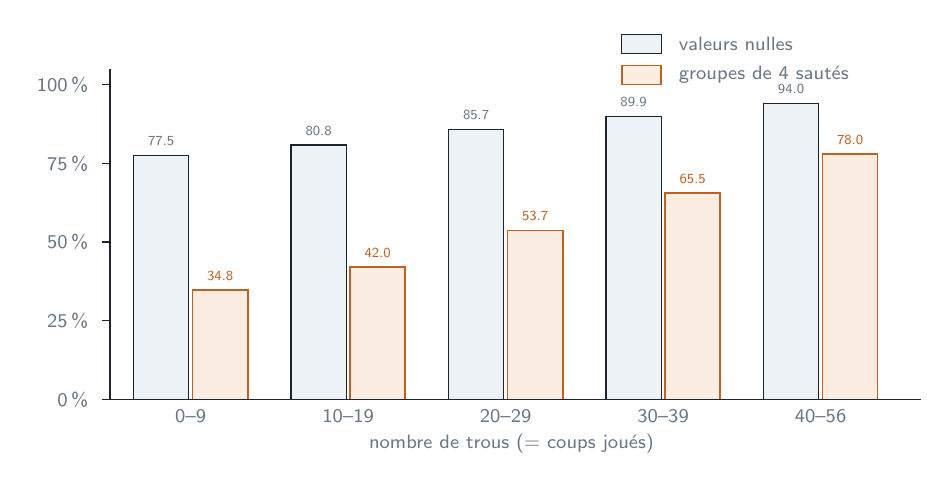
\begin{tikzpicture}[x=1mm,y=0.4mm]
  % groups of 4 entirely zero (skipped) and values zero, by number of holes (measured, current network)
  \foreach \i/\lab/\g/\z in {0/{0–9}/34.8/77.5, 1/{10–19}/42.0/80.8, 2/{20–29}/53.7/85.7, 3/{30–39}/65.5/89.9, 4/{40–56}/78.0/94.0} {
    \pgfmathsetmacro{\x}{20*\i}
    \fill[soft] (\x,0) rectangle ++(7,\z);
    \draw[ink,line width=.4pt] (\x,0) rectangle ++(7,\z);
    \fill[soft2] (\x+7.5,0) rectangle ++(7,\g);
    \draw[accent2,line width=.6pt] (\x+7.5,0) rectangle ++(7,\g);
    \node[font=\sffamily\tiny,text=muted,above] at (\x+3.5,\z) {\z};
    \node[font=\sffamily\tiny,text=accent2,above] at (\x+11,\g) {\g};
    \node[tiny,below] at (\x+7.25,0) {\lab};
  }
  \draw[ink,line width=.6pt] (-3,0) -- (100,0);
  \draw[ink,line width=.6pt] (-3,0) -- (-3,105);
  \foreach \v in {0,25,50,75,100} {
    \draw[ink] (-4,\v) -- (-3,\v);
    \node[tiny,anchor=east] at (-4.5,\v) {\v\,\%};
  }
  \node[tiny] at (48,-14) {nombre de trous (= coups joués)};
  \fill[soft] (62,110) rectangle ++(5,6); \draw[ink,line width=.4pt] (62,110) rectangle ++(5,6);
  \node[tiny,anchor=west] at (68,113) {valeurs nulles};
  \fill[soft2] (62,100) rectangle ++(5,6); \draw[accent2,line width=.6pt] (62,100) rectangle ++(5,6);
  \node[tiny,anchor=west] at (68,103) {groupes de 4 sautés};
\end{tikzpicture}
\end{document}
